

\section{Dataset}
We have collected several sequences with the sensor rig to showcase the system's potential.
The dataset contains the raw data from the cameras, metadata for each frame, and raw data from the \gls{imu} and \gls{gnss} receivers.
The current dataset consists of one sequence where we filmed a moving \gls{usv} from land, one where we recorded data from a moving ship driving in the city canal, and two scenes where we walked along the river and filmed the water surface from different angles.
We plan on expanding the data set by adding more scenarios in the future.
As we want to ensure quality before releasing calibration data, we also provide a calibration sequence where we film a chess board while rapidly moving the sensor rig, which can be used for calibration purposes.
The following images are a representative selection from the datasets, showing the $S0$ image on the left, which is what a regular camera would capture, and a visualization of polarization information on the right.

The dataset is available at \url{https://github.com/emillma/sensor-rig-datasets}.

\begin{figure}[H]
    \begin{subfigure}[T]{.49\textwidth}
        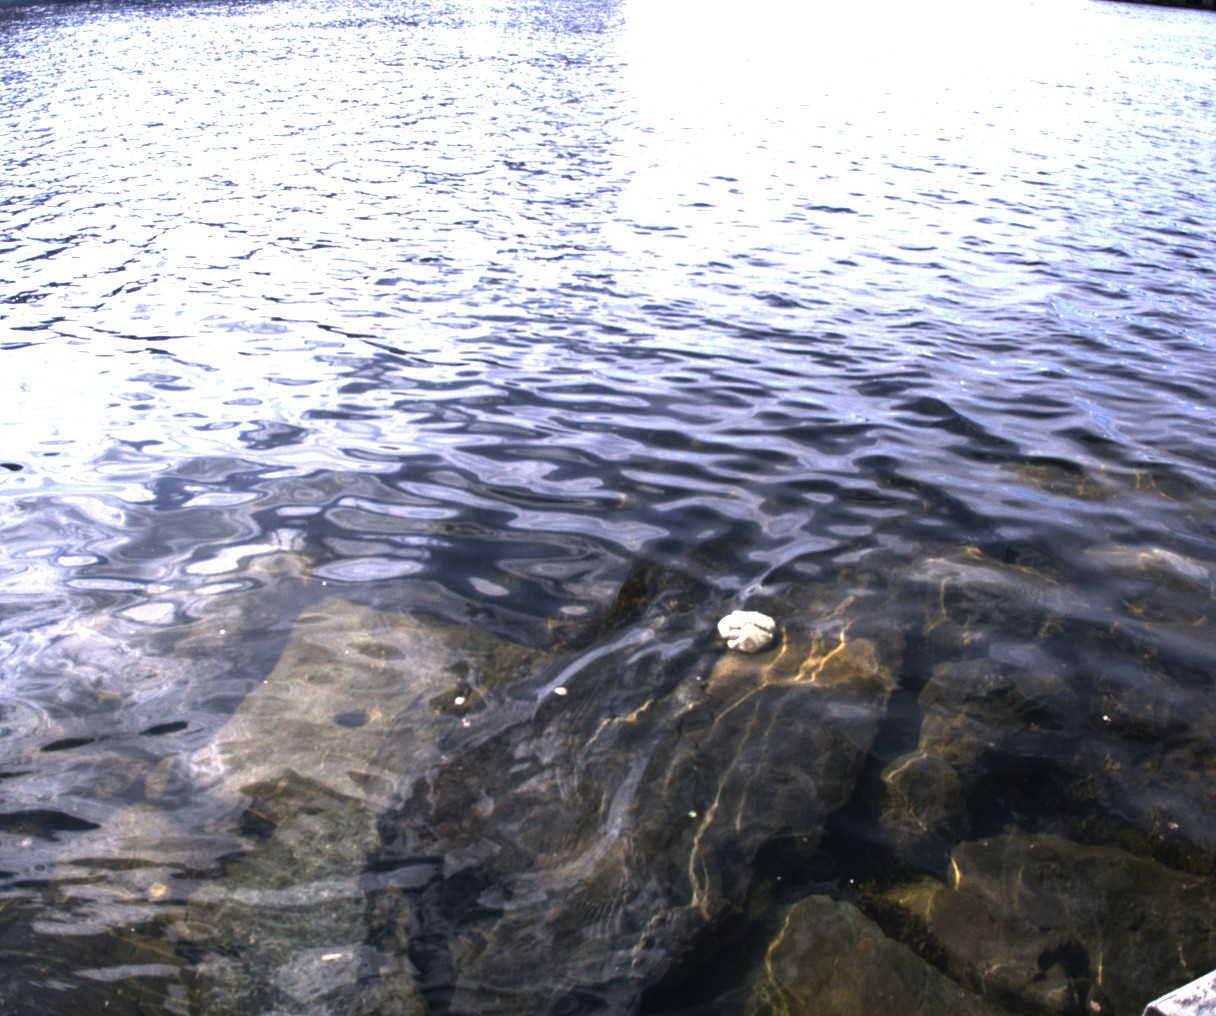
\includegraphics[width=\textwidth]{figures/pictures/img_4722_s0.jpg}
    \end{subfigure} \hfill
    \begin{subfigure}[T]{.49\textwidth}
        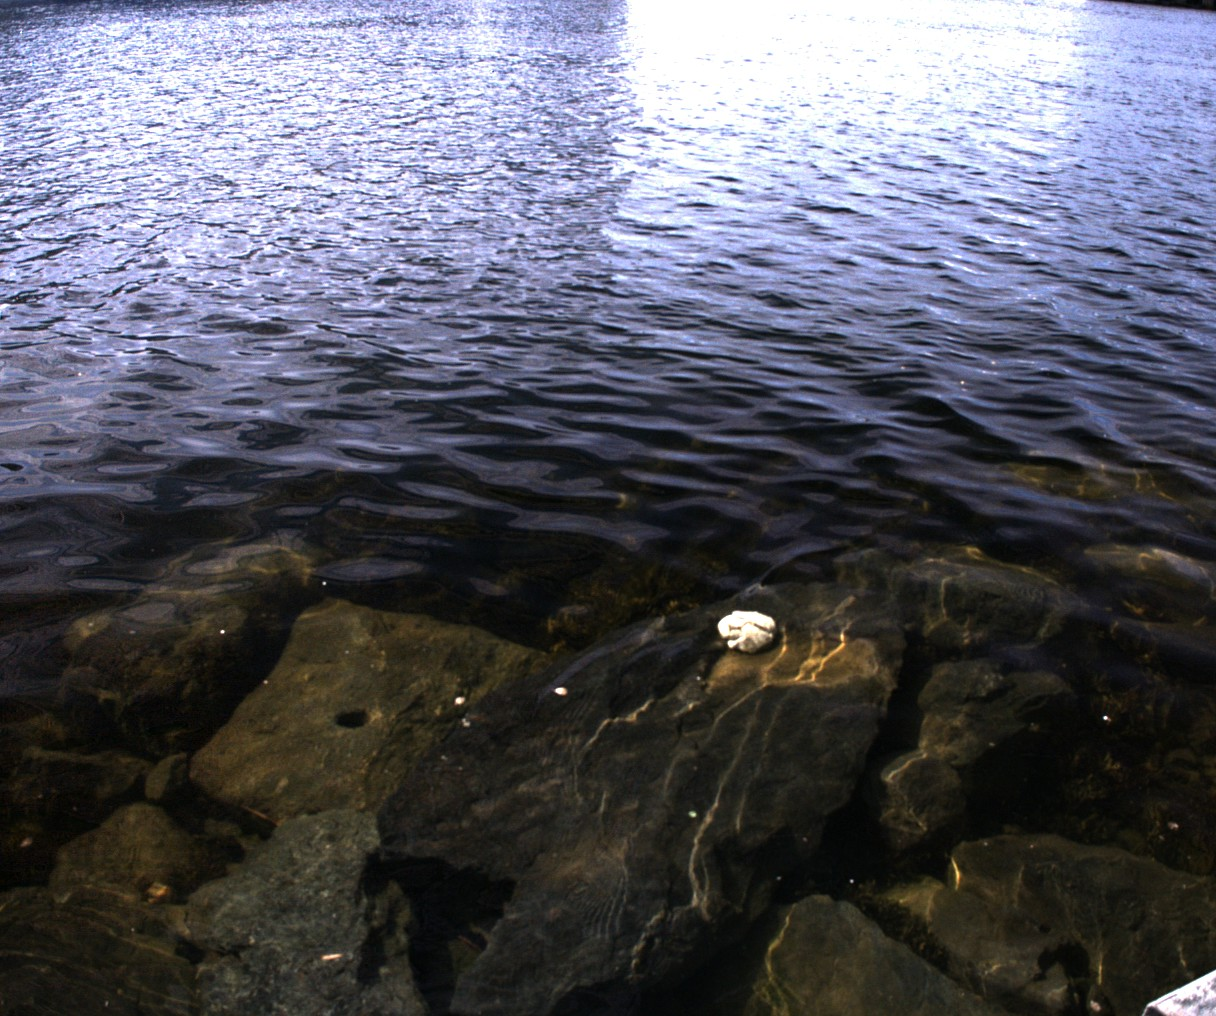
\includegraphics[width=\textwidth]{figures/pictures/img_4722_unpol.jpg}
    \end{subfigure}
    \caption{Image where the linearly polarized light is removed to remove glare and improve sub-surface visibility. Note that the degree to which reflections are removed follows Figure \ref{fig:dolp_graph}.
    }
\end{figure}
\vspace{-.5cm}

\begin{figure}[H]
    \begin{subfigure}[T]{.49\textwidth}
        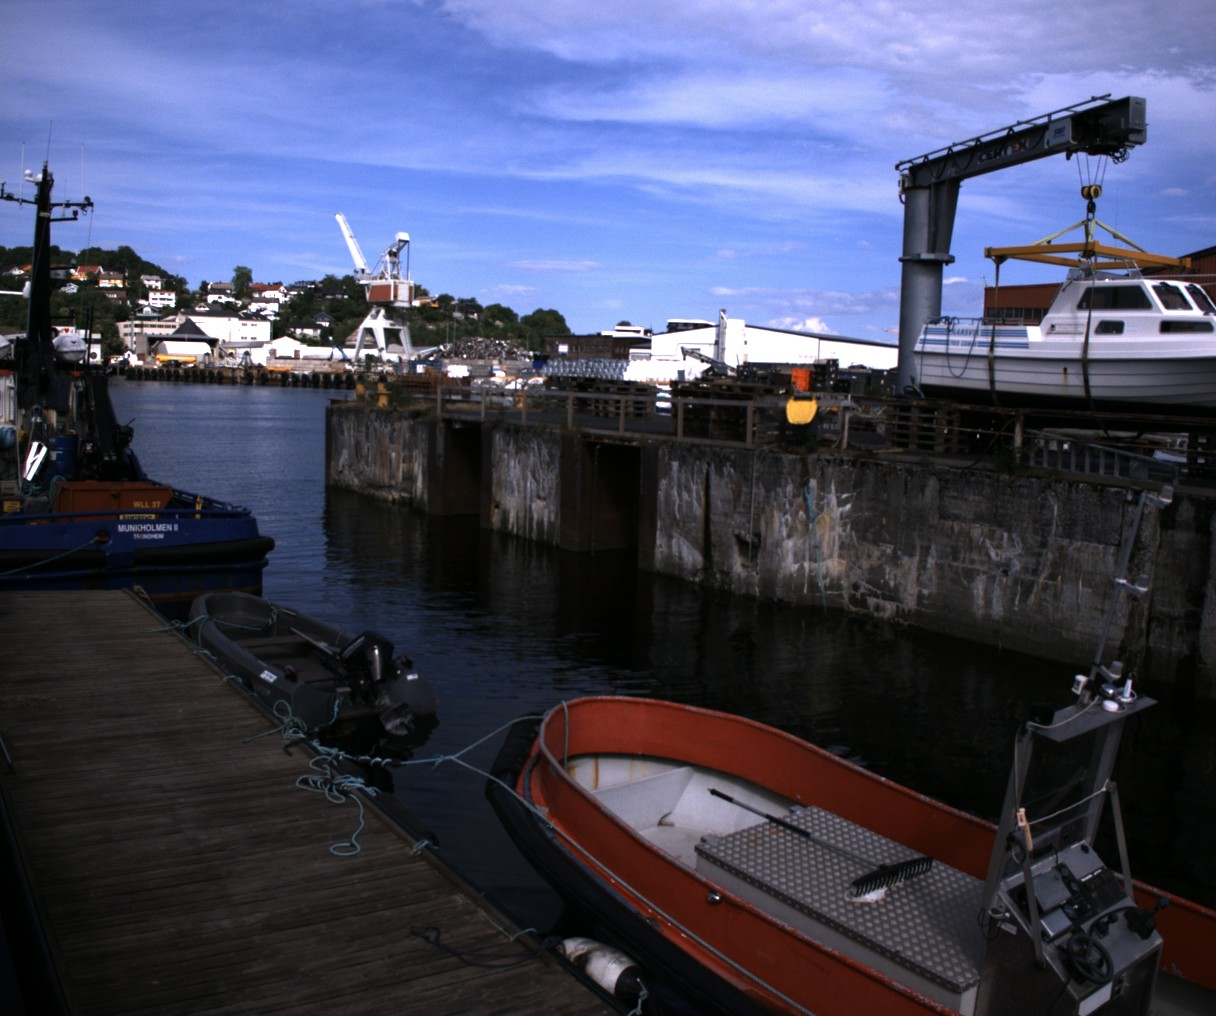
\includegraphics[width=\textwidth]{figures/pictures/img_2790_s0.jpg}
    \end{subfigure} \hfill
    \begin{subfigure}[T]{.49\textwidth}
        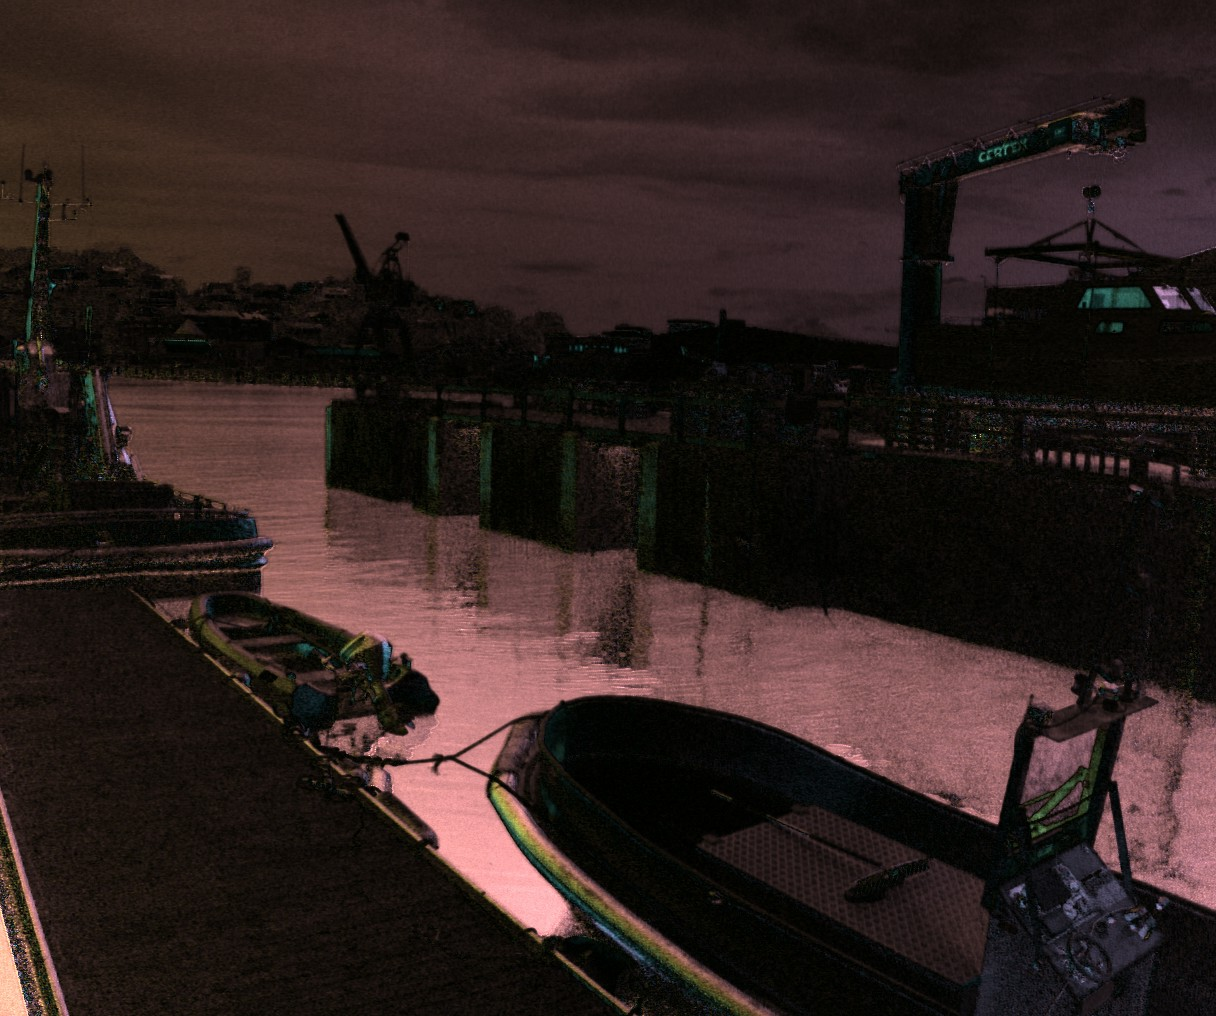
\includegraphics[width=\textwidth]{figures/pictures/img_2790_pol.jpg}
    \end{subfigure}
    \caption{Docking area demonstrating how the polarization of the water surface makes it more visible. 
    The visualization and color map of this figure and the following figures are equivalent to Figure \ref{fig:cpfa_demosaicking}.}
\end{figure}
\vspace{-.7cm}

\begin{figure}[H]
    \begin{subfigure}[T]{.49\textwidth}
        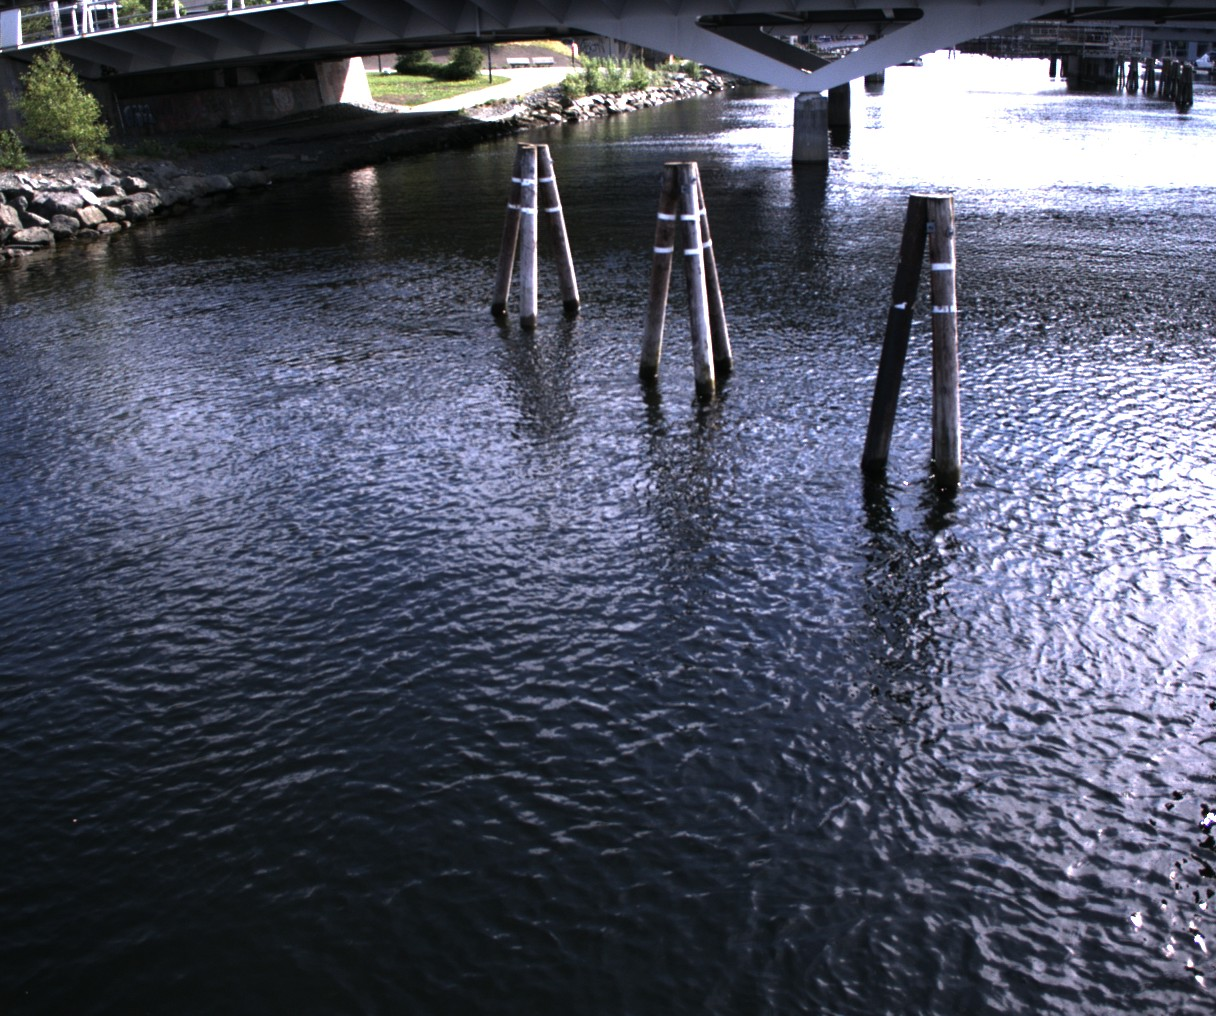
\includegraphics[width=\textwidth]{figures/pictures/img_7458_s0.jpg}
    \end{subfigure} \hfill
    \begin{subfigure}[T]{.49\textwidth}
        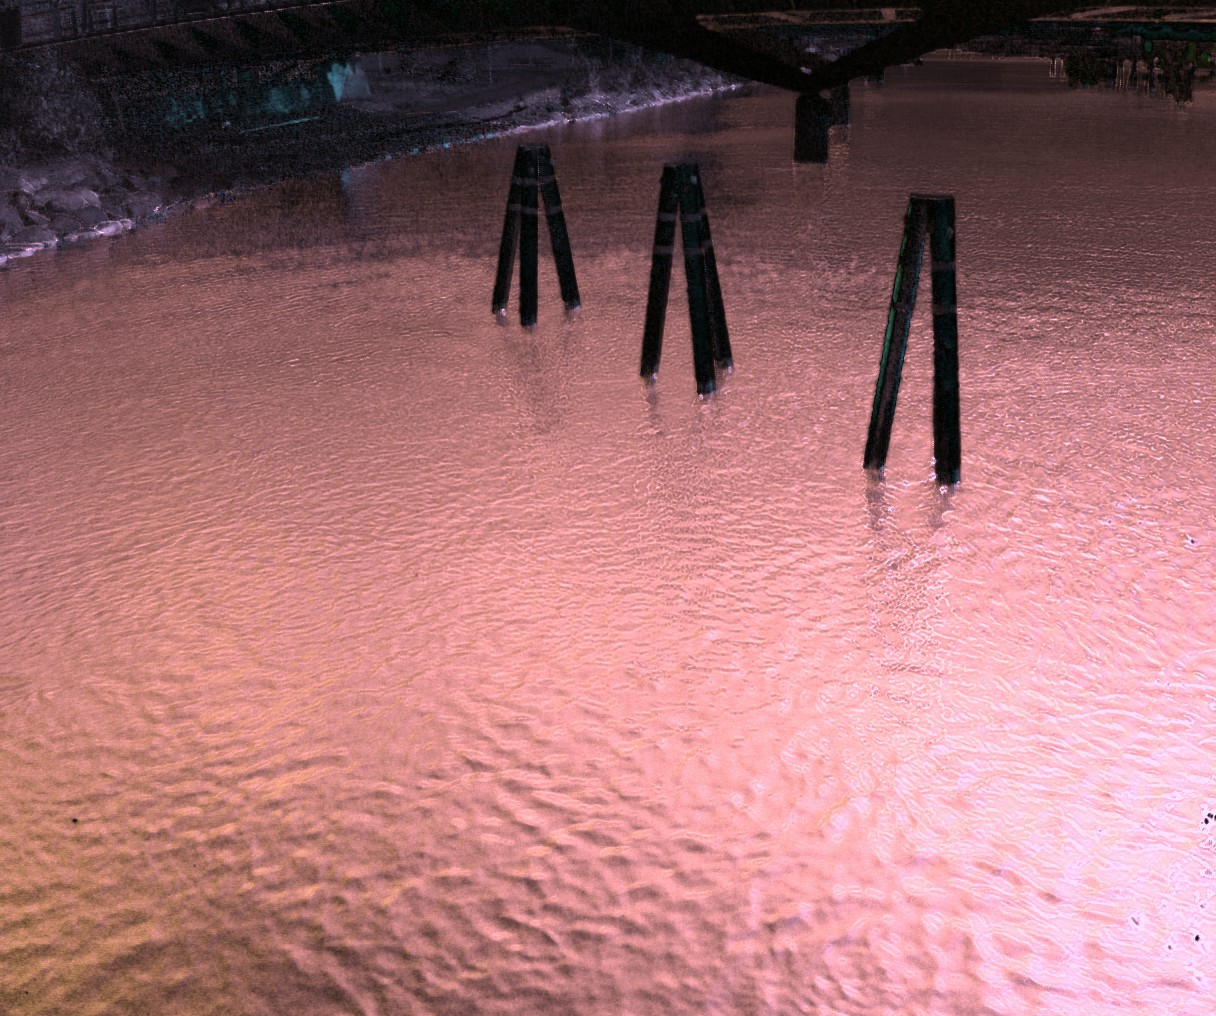
\includegraphics[width=\textwidth]{figures/pictures/img_7458_pol.jpg}
    \end{subfigure}
    \caption{Wooden posts protruding from the water.}
\end{figure}
\vspace{-.5cm}

\begin{figure}[H]
    \begin{subfigure}[T]{.49\textwidth}
        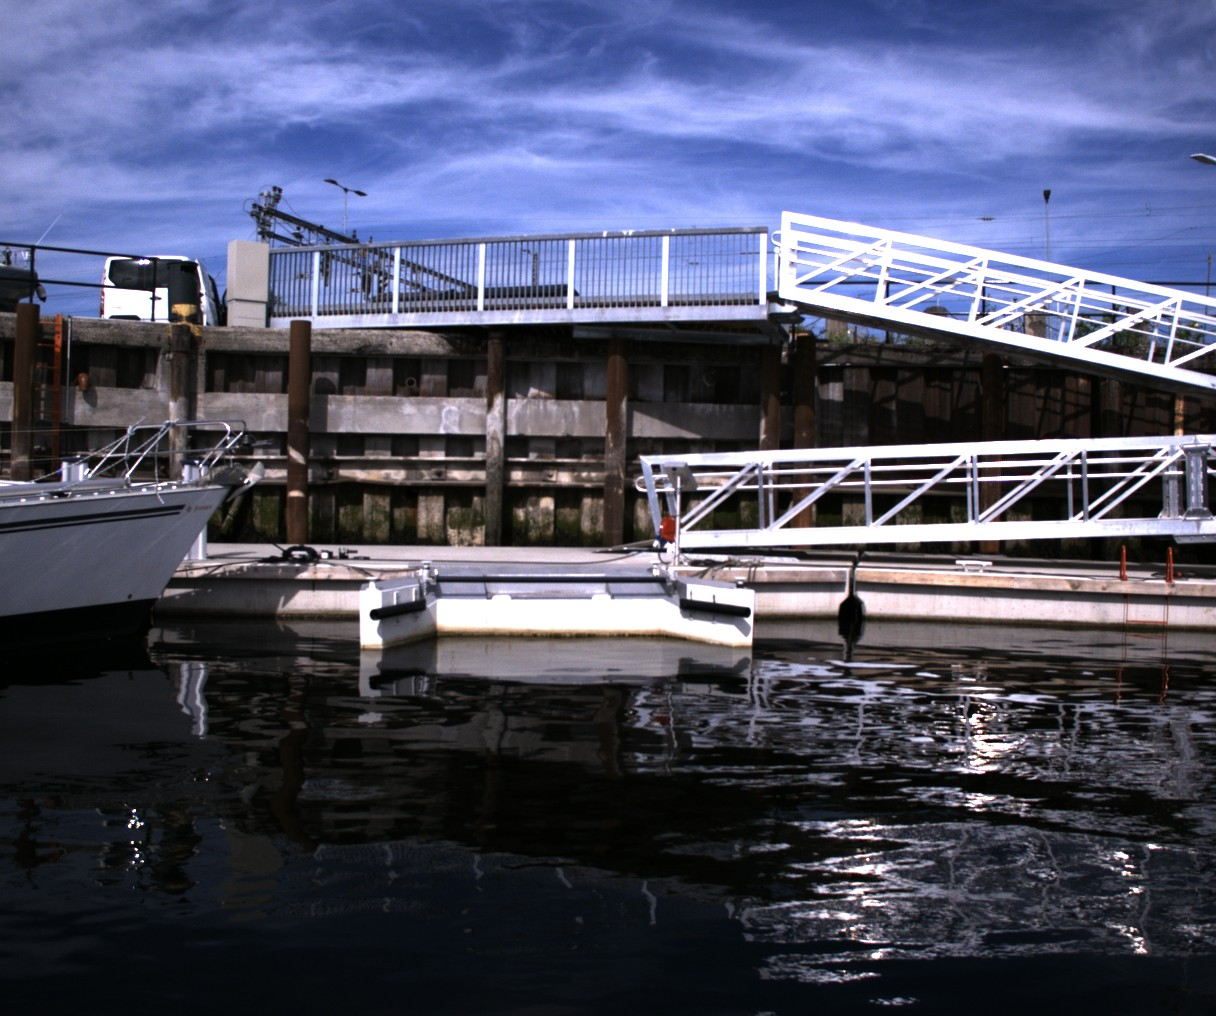
\includegraphics[width=\textwidth]{figures/pictures/img_11640_s0.jpg}
    \end{subfigure} \hfill
    \begin{subfigure}[T]{.49\textwidth}
        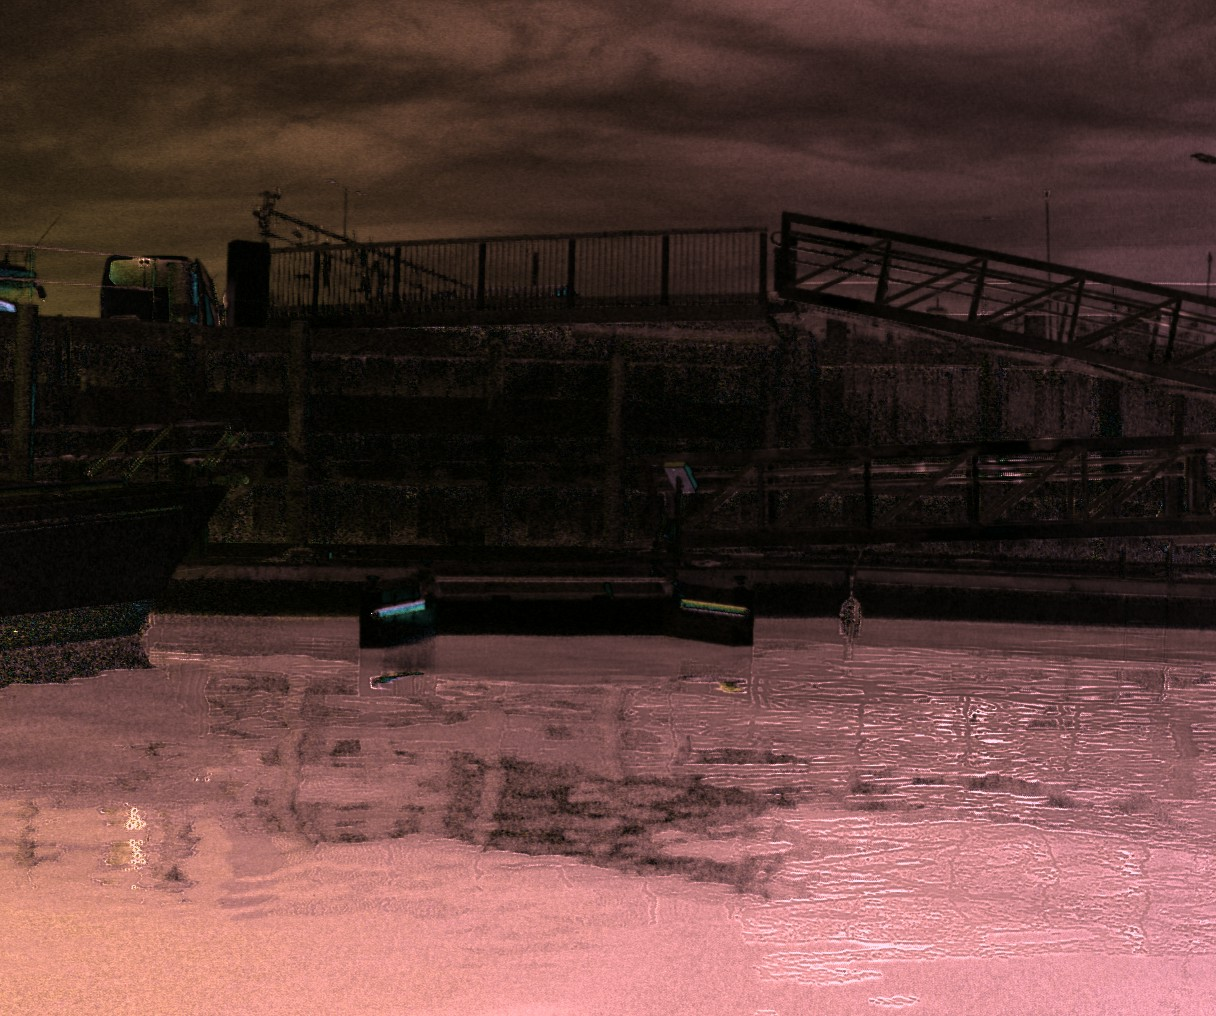
\includegraphics[width=\textwidth]{figures/pictures/img_11640_pol.jpg}
    \end{subfigure}
    \caption{View from a moving vessel approaching the dock.}
\end{figure}
\vspace{-.5cm}

\begin{figure}[H]
    \begin{subfigure}[T]{.49\textwidth}
        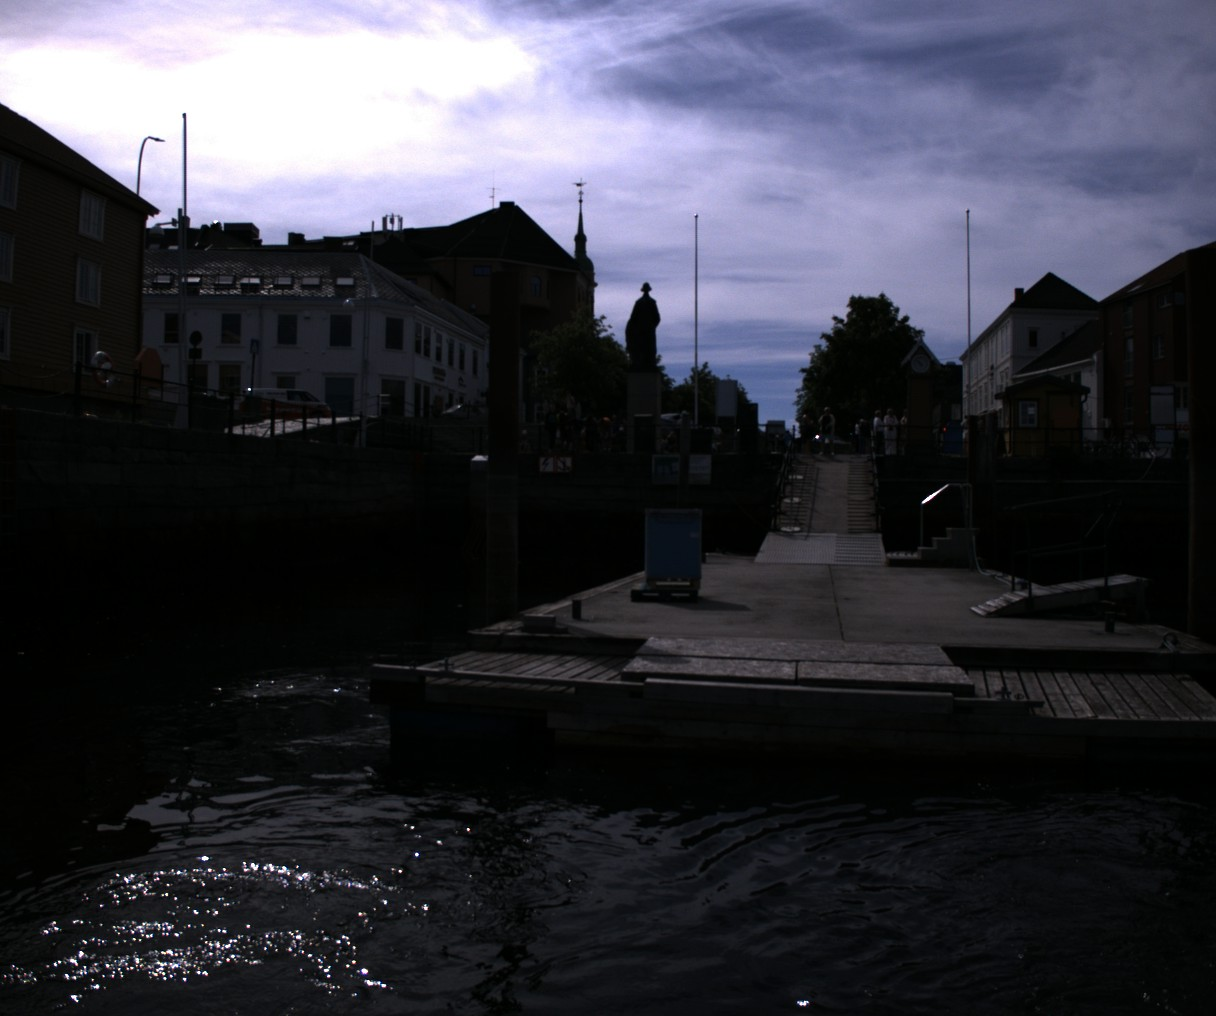
\includegraphics[width=\textwidth]{figures/pictures/img_10170_s0.jpg}
    \end{subfigure} \hfill
    \begin{subfigure}[T]{.49\textwidth}
        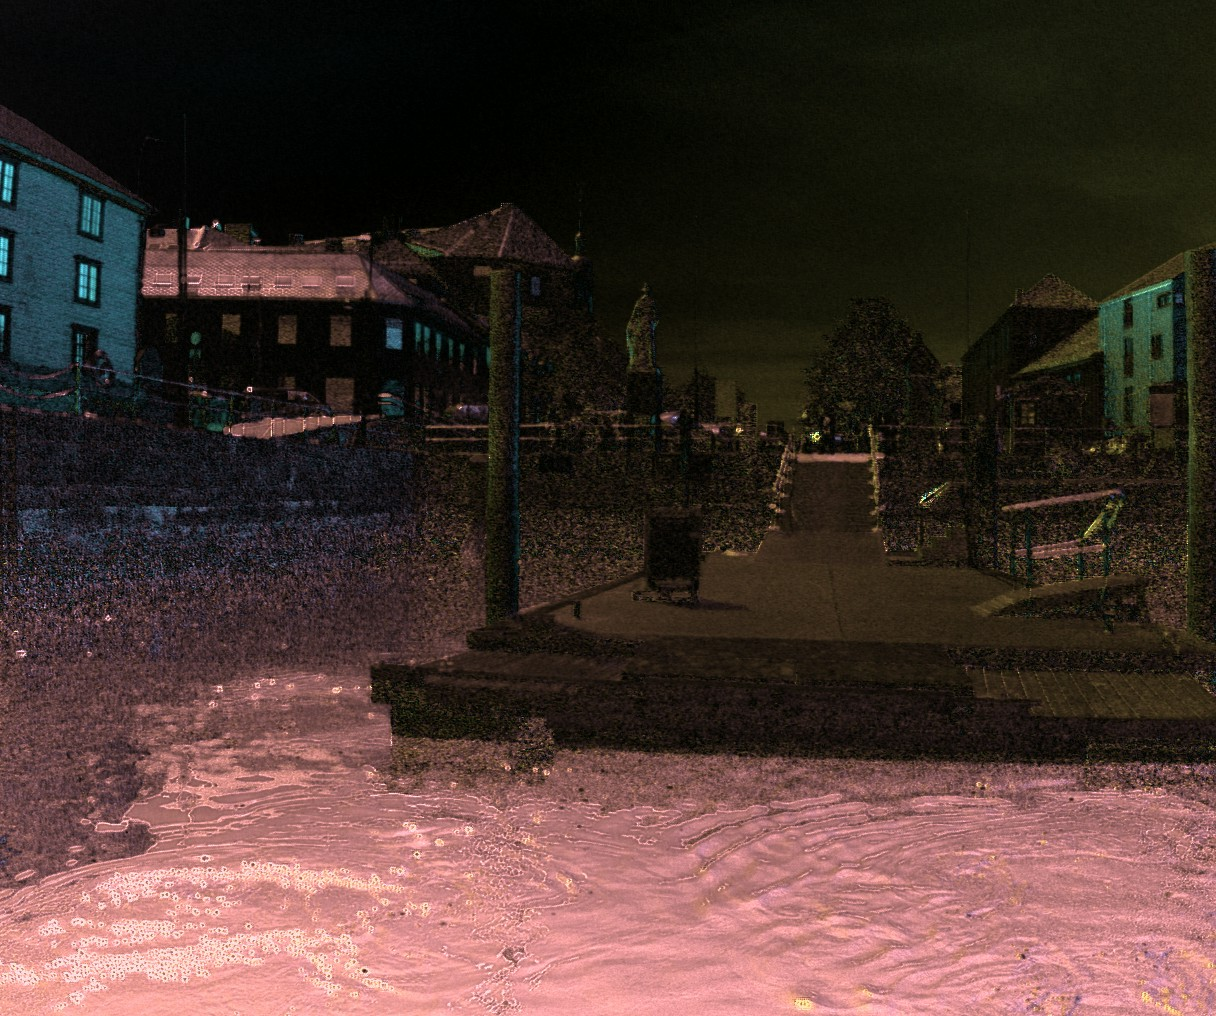
\includegraphics[width=\textwidth]{figures/pictures/img_10170_pol.jpg}
    \end{subfigure}
    \caption{Underexposed image of a dock viewed from the water.}
\end{figure}
\vspace{-.5cm}


\begin{figure}[H]
    \begin{subfigure}[T]{.49\textwidth}
        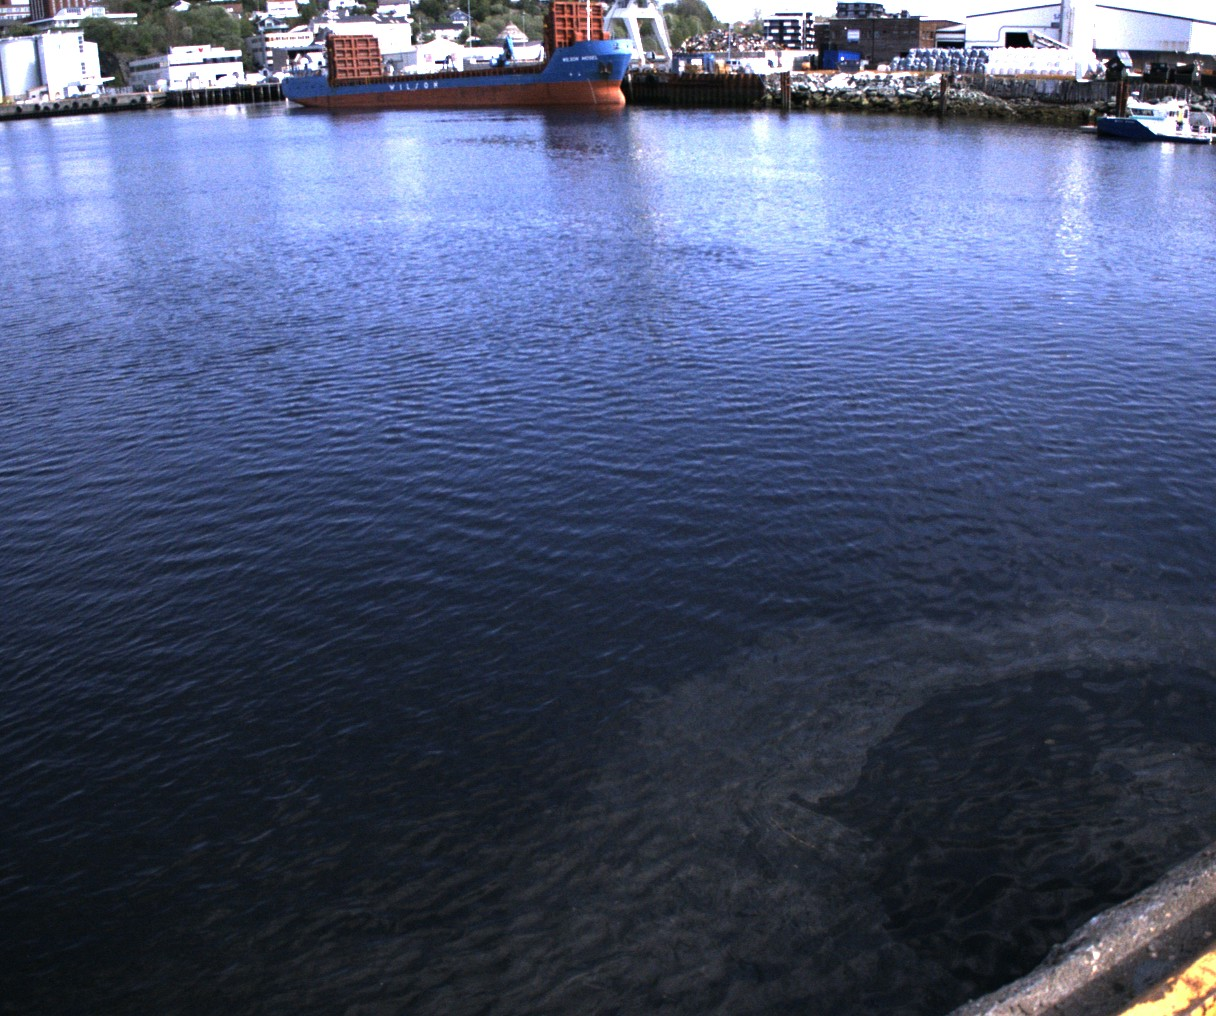
\includegraphics[width=\textwidth]{figures/pictures/img_3726_s0.jpg}
    \end{subfigure} \hfill
    \begin{subfigure}[T]{.49\textwidth}
        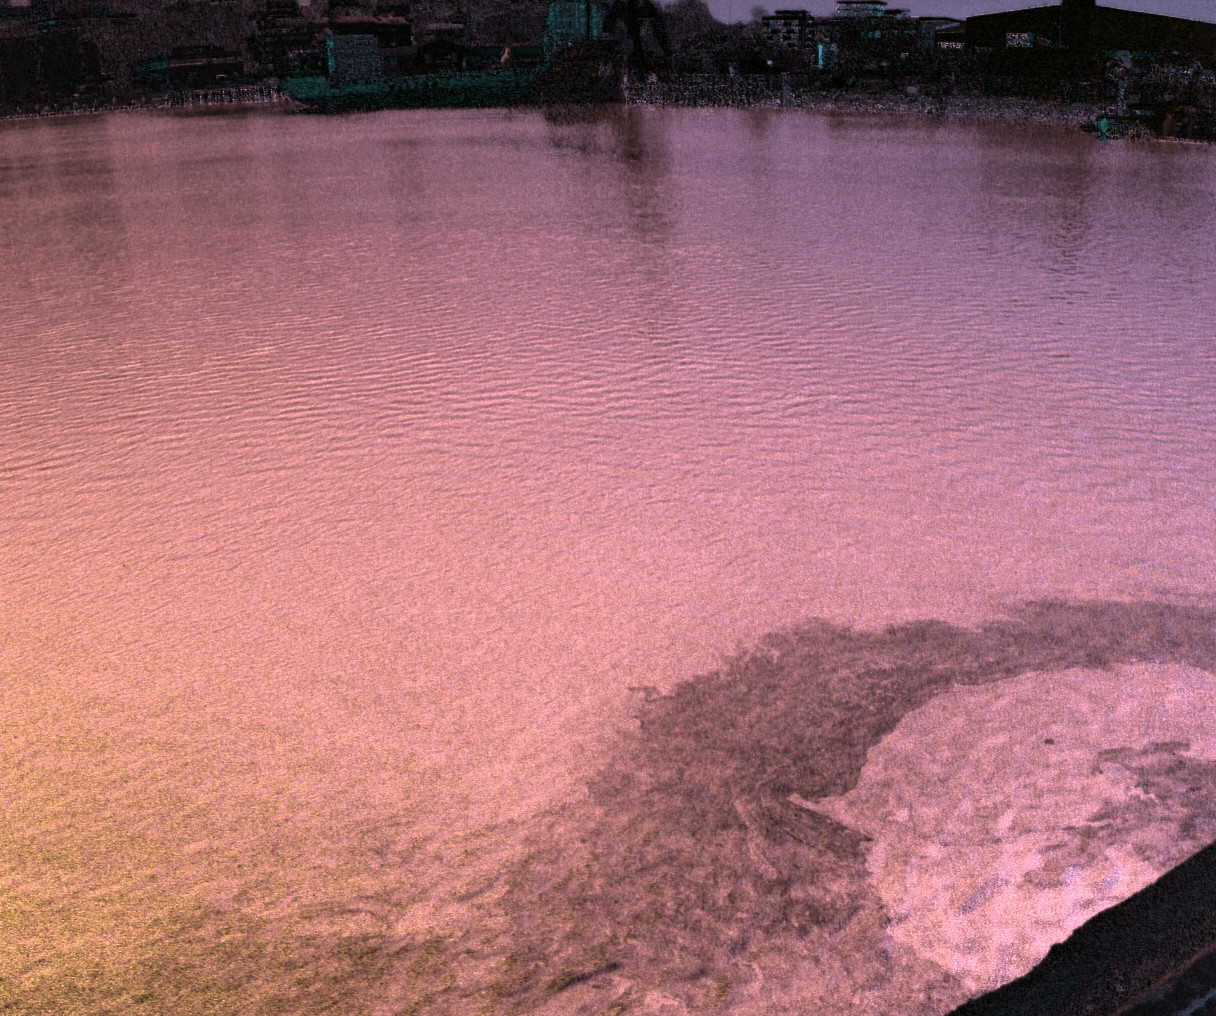
\includegraphics[width=\textwidth]{figures/pictures/img_3726_pol.jpg}
    \end{subfigure}
    \caption{Pollen on the water surface.}
\end{figure}
\vspace{-.5cm}

\begin{figure}[H]
    \begin{subfigure}[T]{.49\textwidth}
        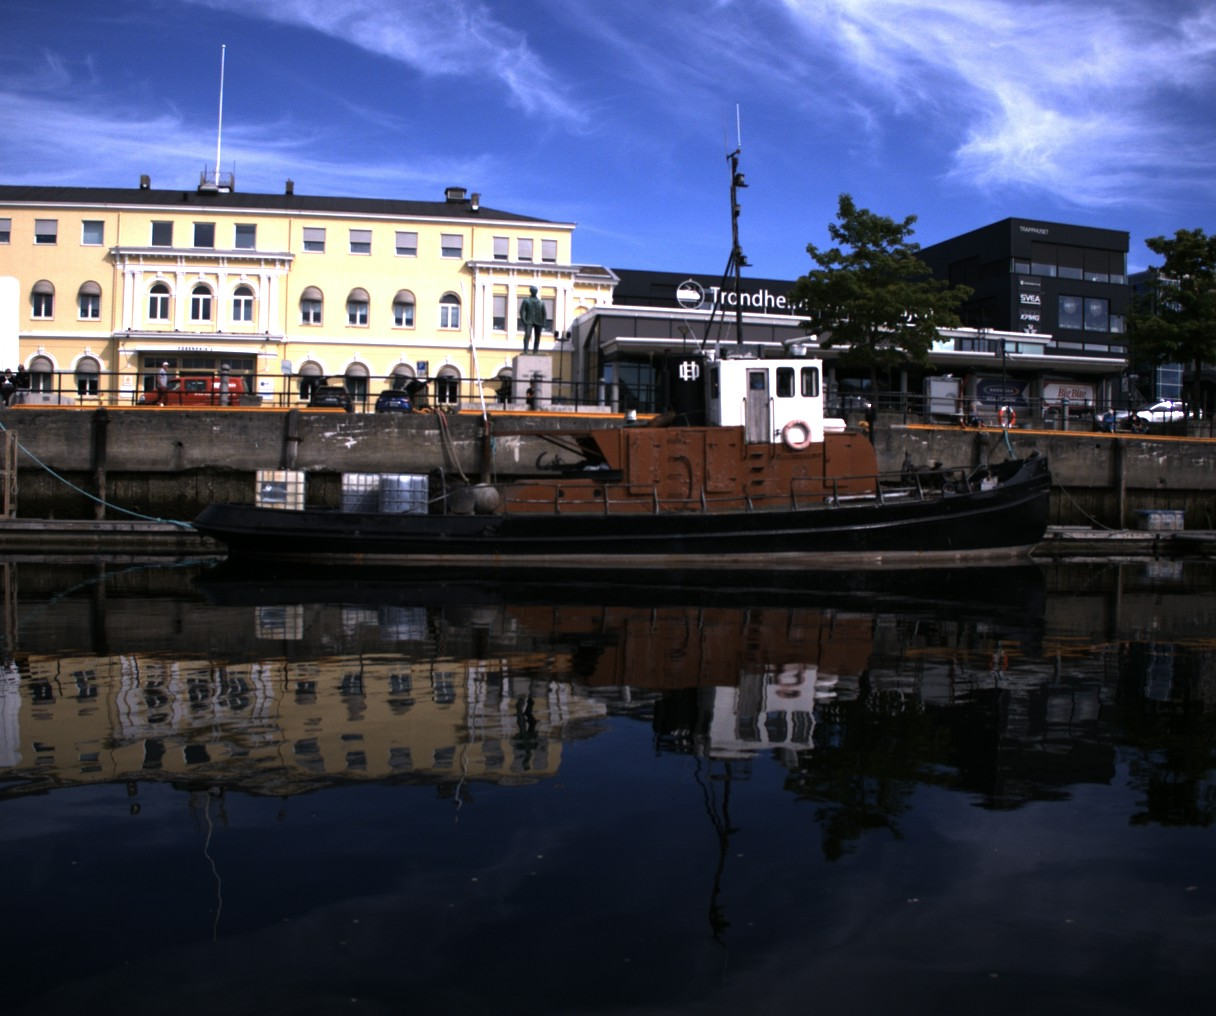
\includegraphics[width=\textwidth]{figures/pictures/img_4038_s0.jpg}
    \end{subfigure} \hfill
    \begin{subfigure}[T]{.49\textwidth}
        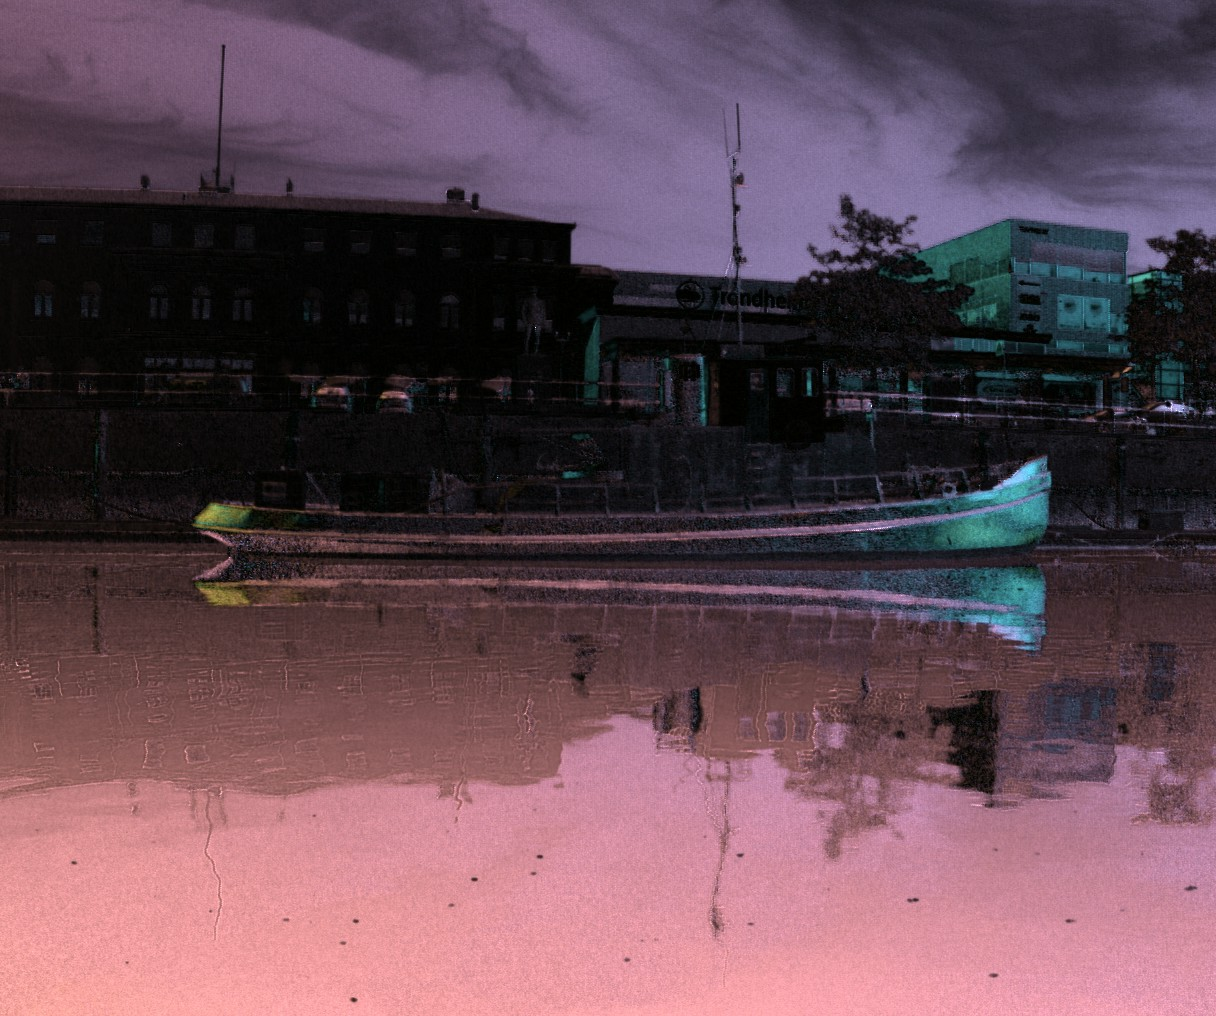
\includegraphics[width=\textwidth]{figures/pictures/img_4038_pol.jpg}
    \end{subfigure}
    \caption{A docked boat viewed from the water.}
\end{figure}
\vspace{-.5cm}

% \begin{figure}[H]
%     \begin{subfigure}[T]{.49\textwidth}
%         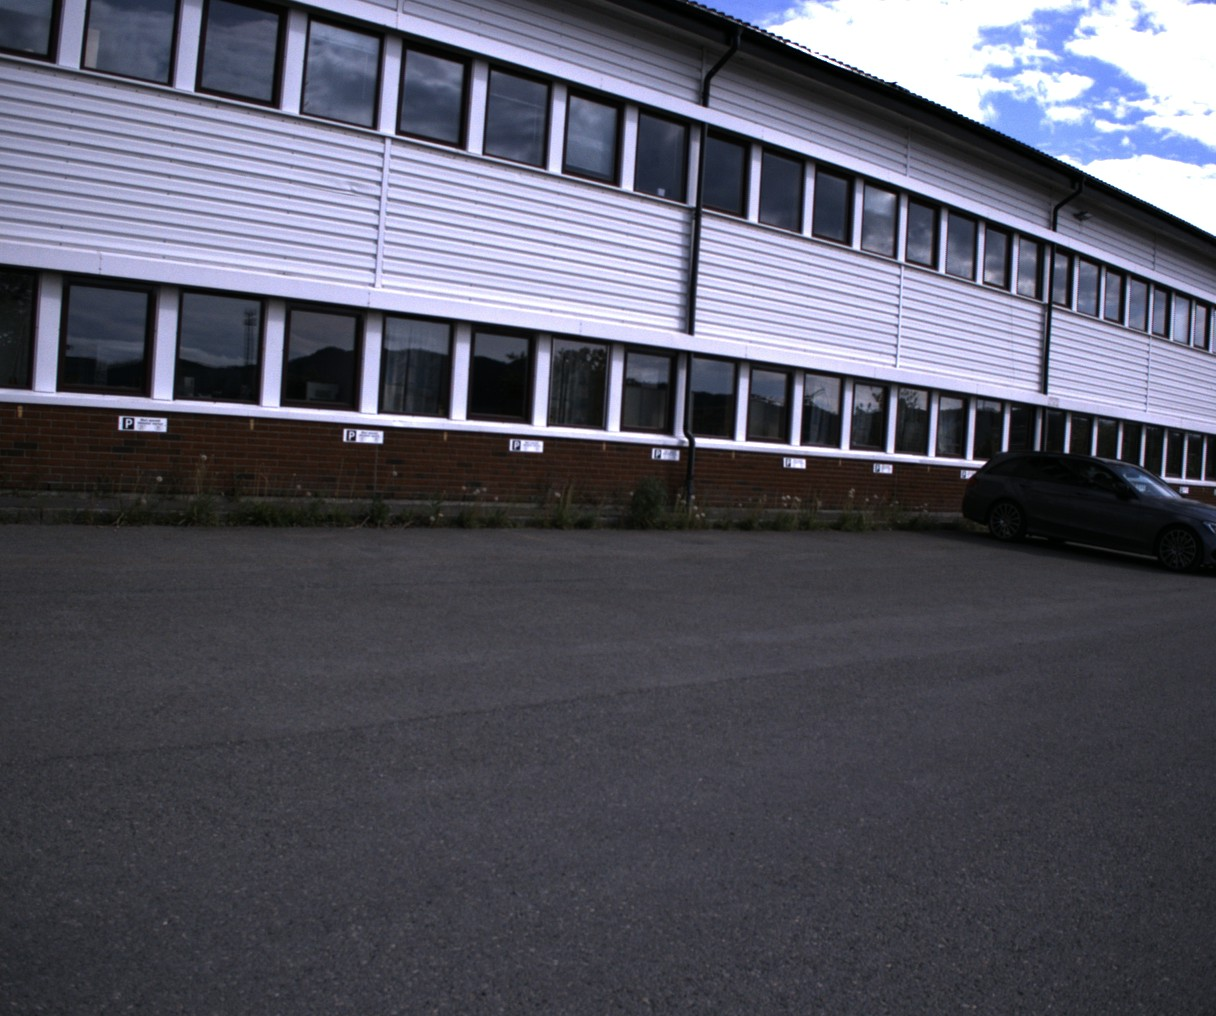
\includegraphics[width=\textwidth]{figures/pictures/img_5742_s0.jpg}
%     \end{subfigure} \hfill
%     \begin{subfigure}[T]{.49\textwidth}
%         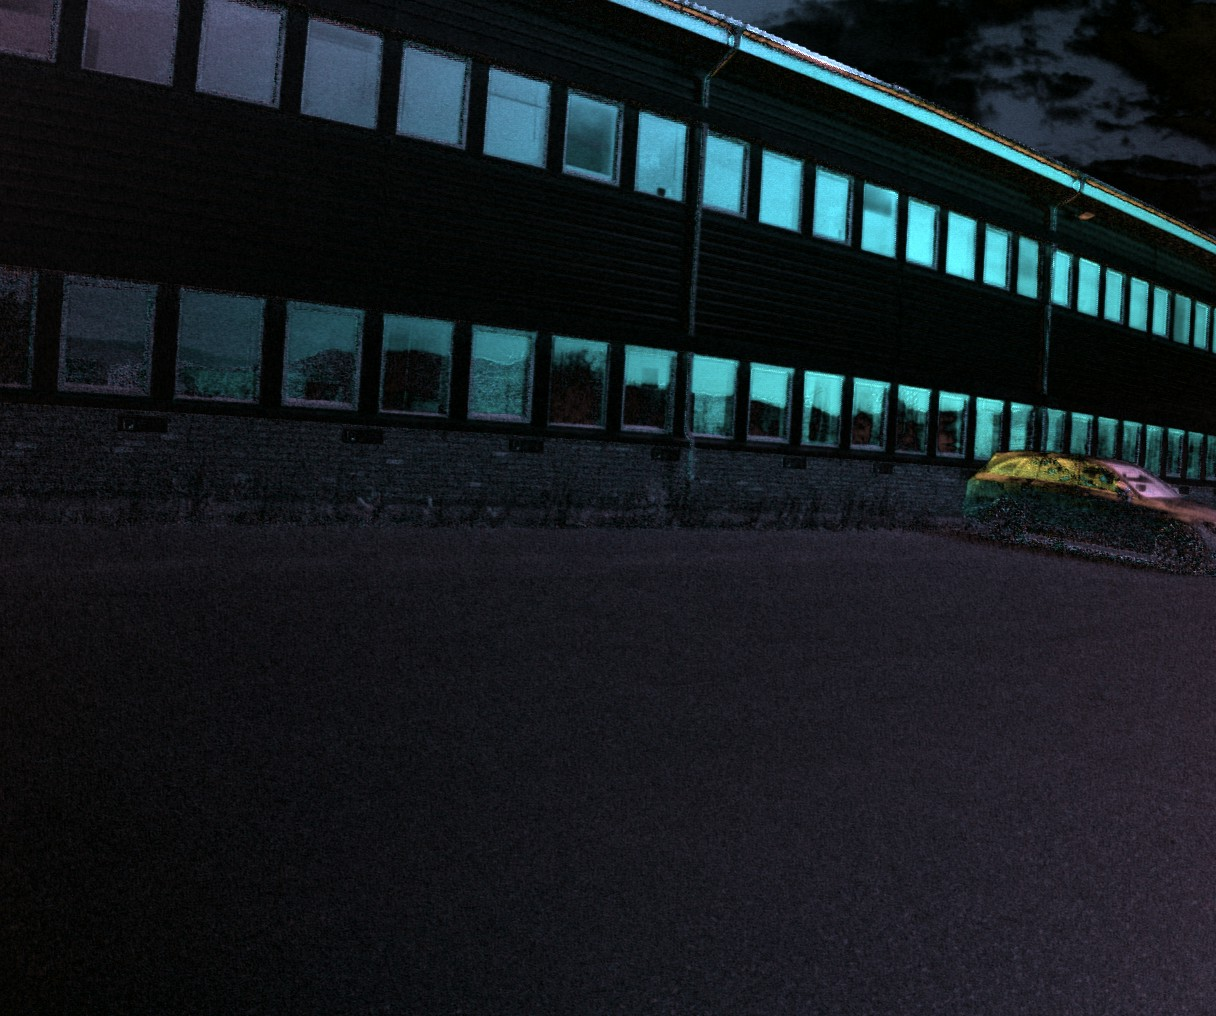
\includegraphics[width=\textwidth]{figures/pictures/img_5742_pol.jpg}
%     \end{subfigure}
%     \caption{Building with glass windows.}
% \end{figure}
% \vspace{-.5cm}
\begin{figure}[H]
    \begin{subfigure}[T]{.49\textwidth}
        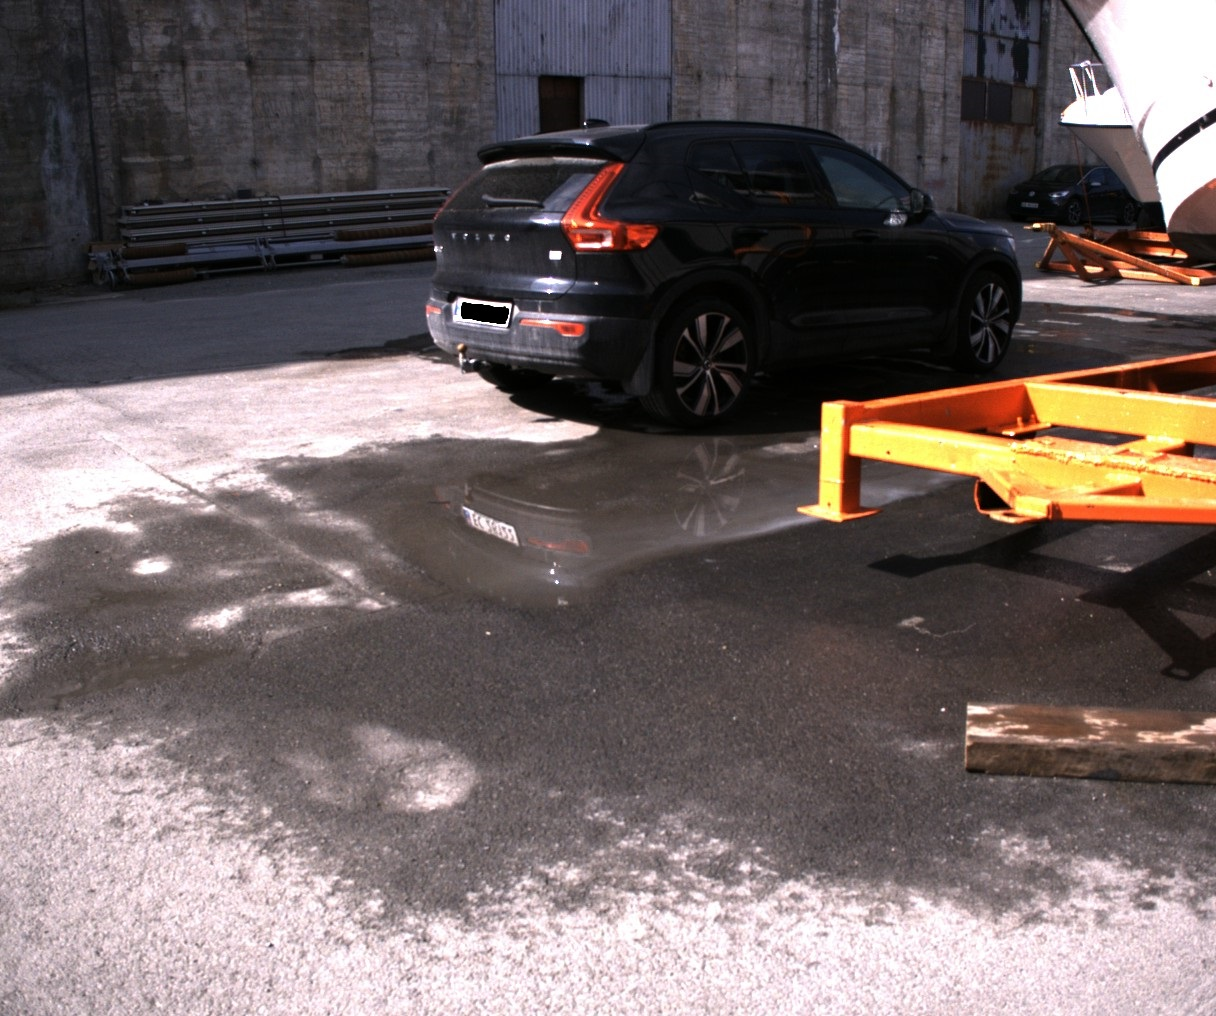
\includegraphics[width=\textwidth]{figures/pictures/img_1116_s0.jpg}
    \end{subfigure} \hfill
    \begin{subfigure}[T]{.49\textwidth}
        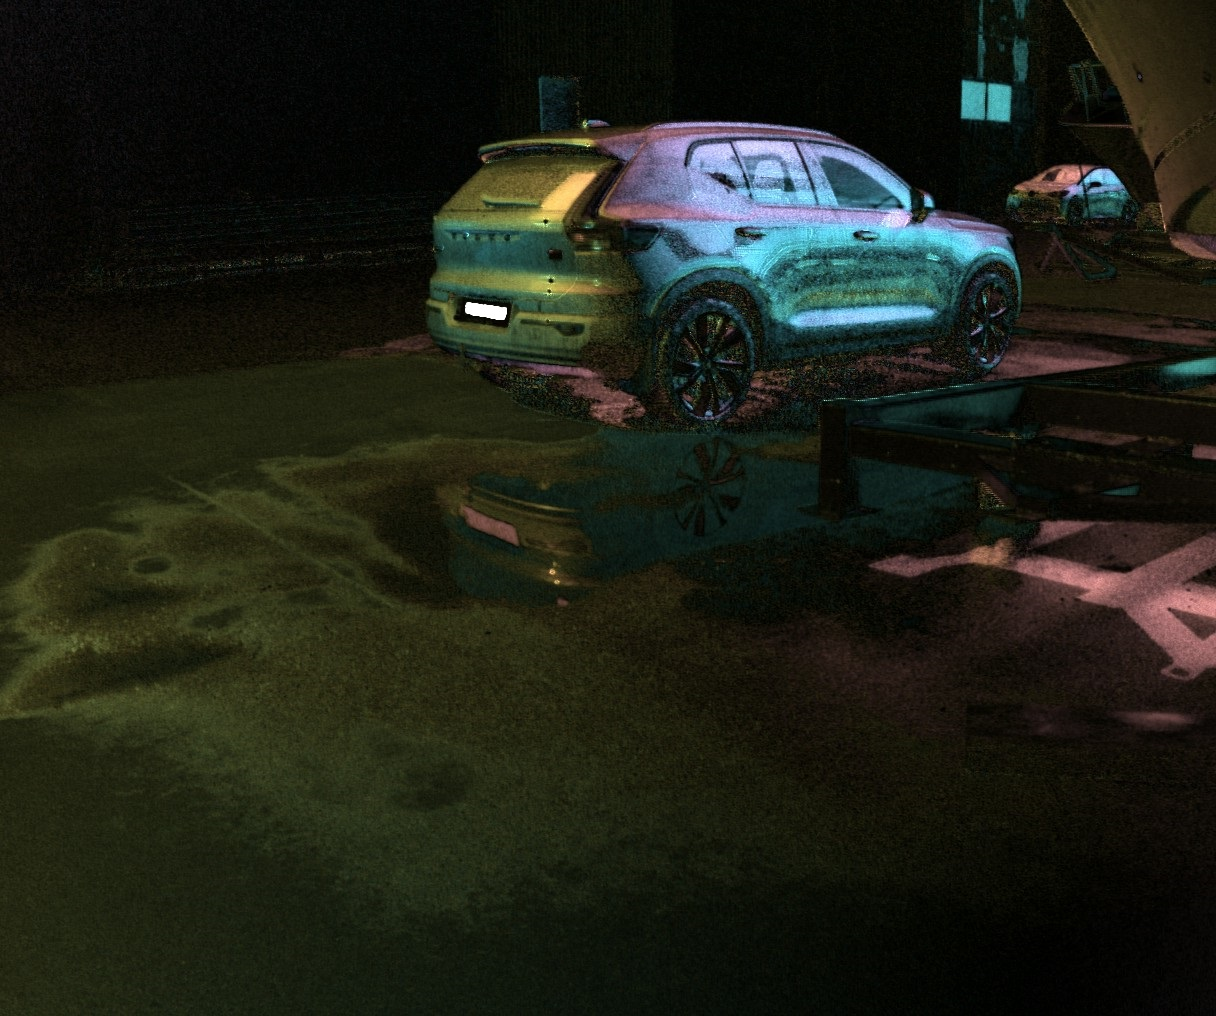
\includegraphics[width=\textwidth]{figures/pictures/img_1116_pol.jpg}
    \end{subfigure}
    \caption{A black car.}
\end{figure}
\vspace{-.5cm}


\begin{figure}[H]
    \begin{subfigure}[T]{.49\textwidth}
        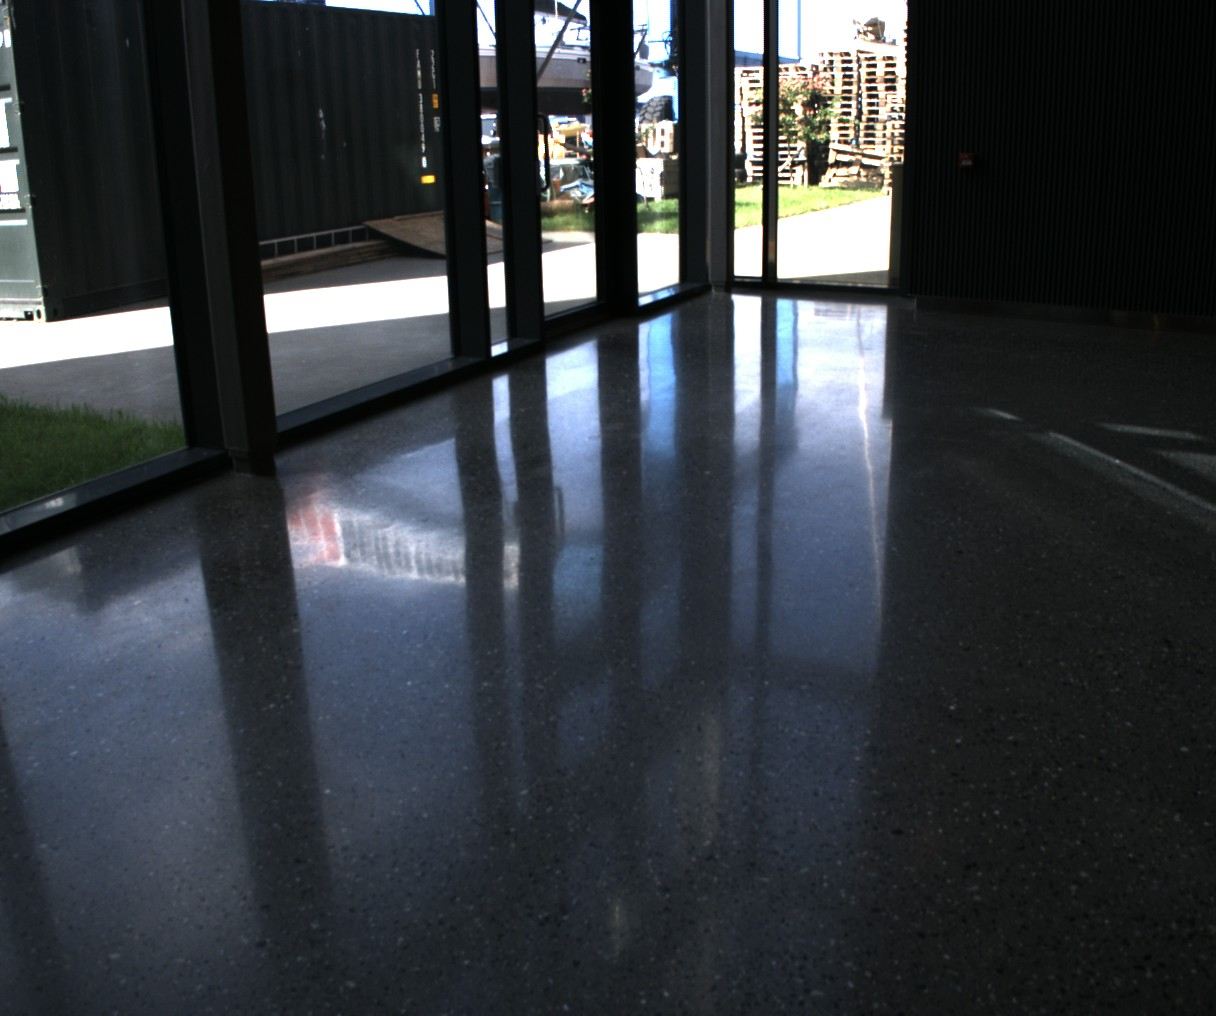
\includegraphics[width=\textwidth]{figures/pictures/img_9222_s0.jpg}
    \end{subfigure} \hfill
    \begin{subfigure}[T]{.49\textwidth}
        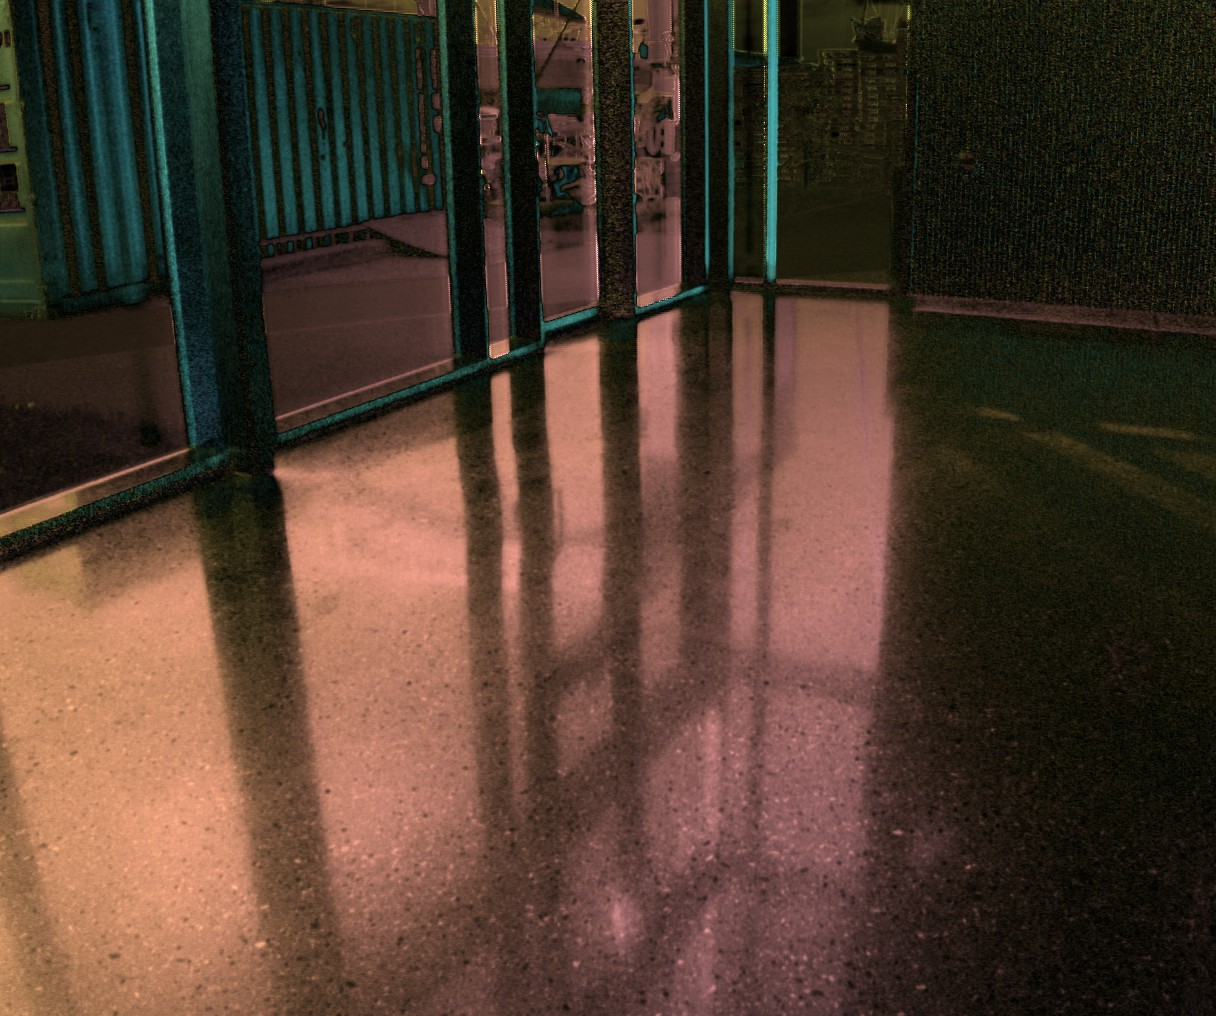
\includegraphics[width=\textwidth]{figures/pictures/img_9222_pol.jpg}
    \end{subfigure}
    \caption{Stone floor with reflections.}
\end{figure}
\vspace{-.5cm}

 \begin{figure}[H]
     \begin{subfigure}[T]{.49\textwidth}
         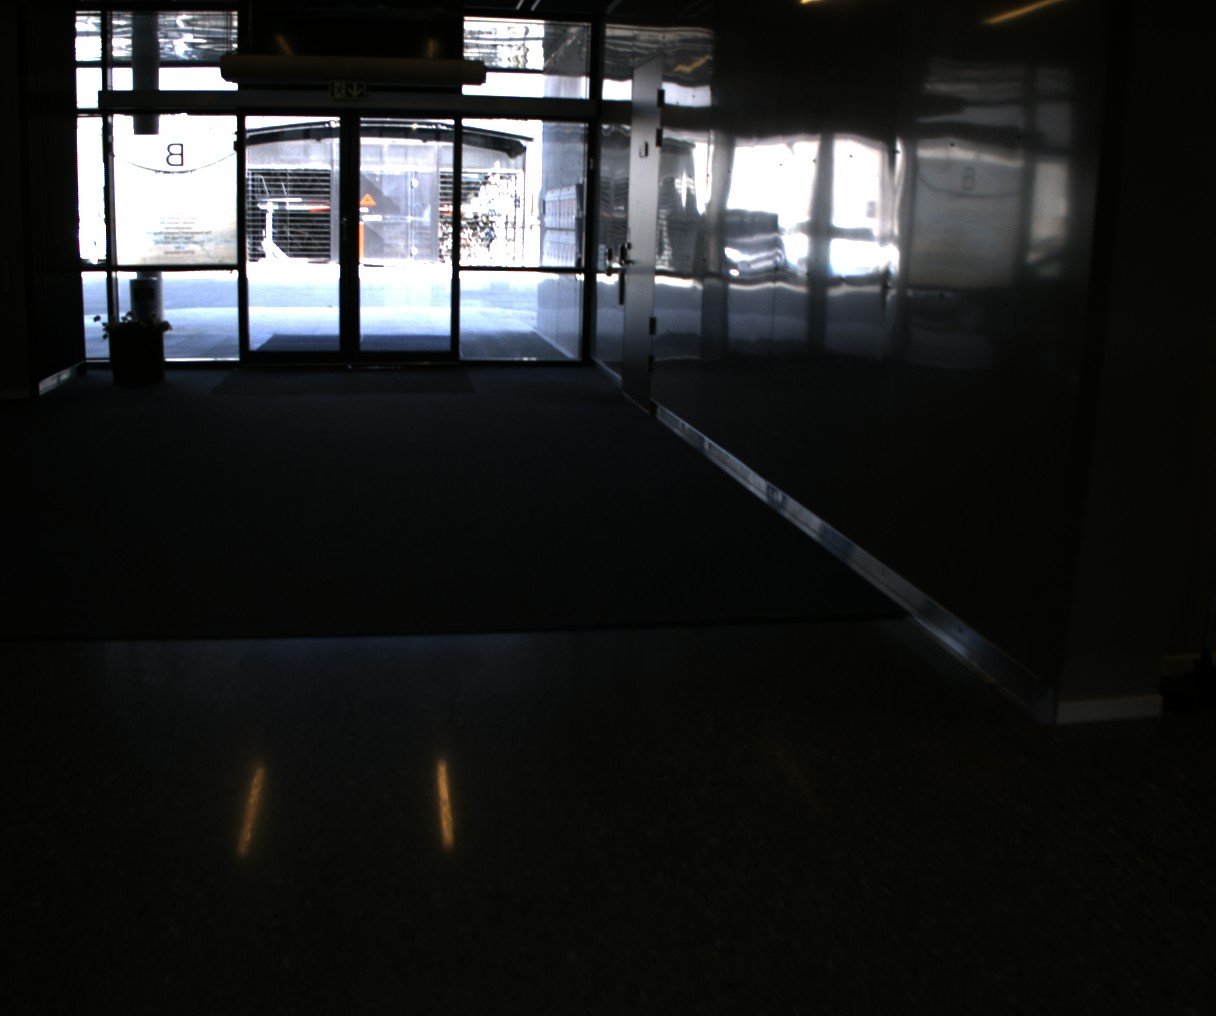
\includegraphics[width=\textwidth]{figures/pictures/img_9306_s0.jpg}
     \end{subfigure} \hfill
    \begin{subfigure}[T]{.49\textwidth}
         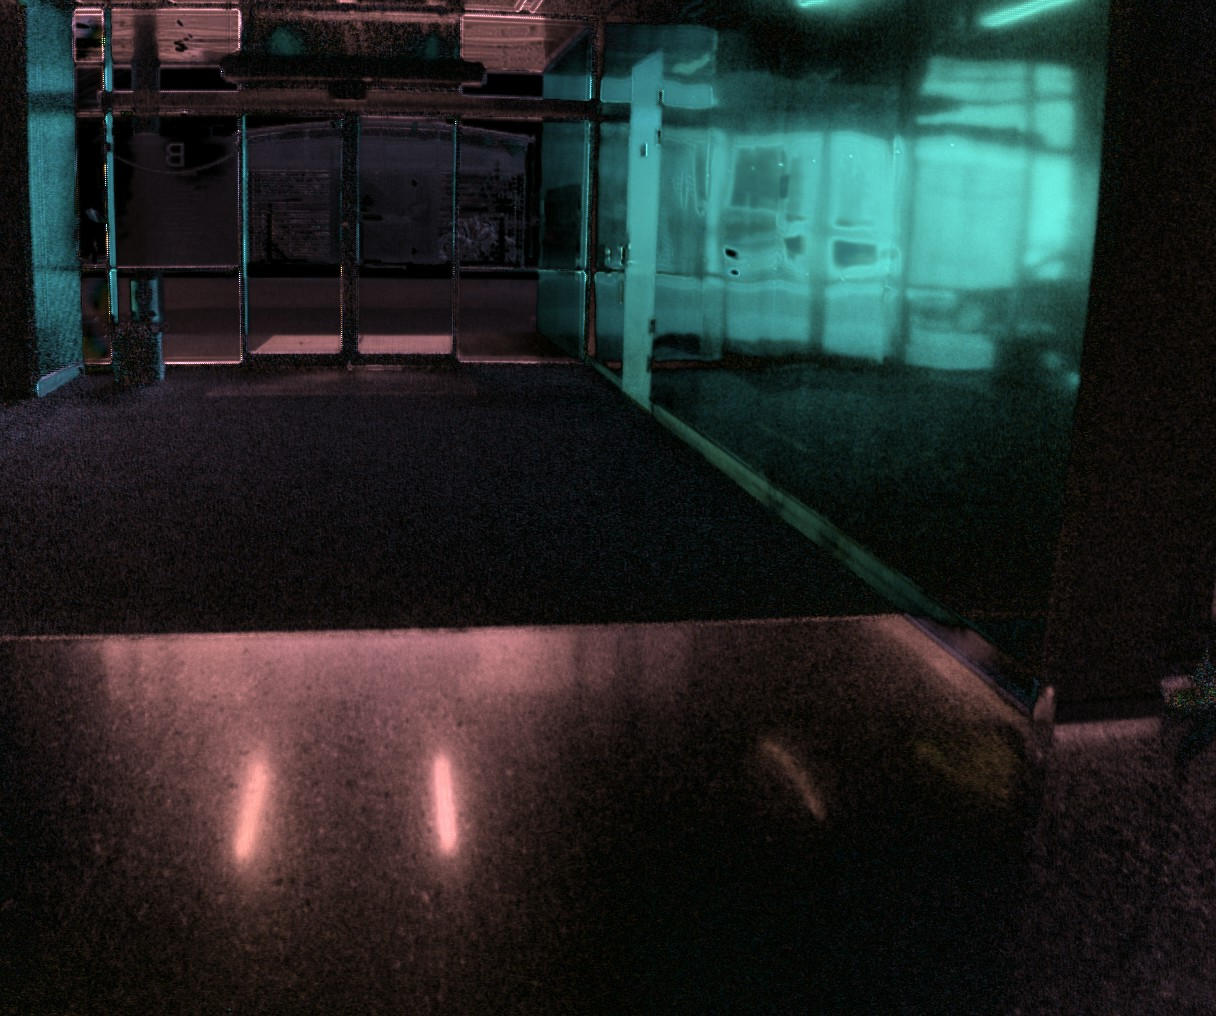
\includegraphics[width=\textwidth]{figures/pictures/img_9306_pol.jpg}
     \end{subfigure}
     \caption{High contrast reflective indoor environment.}
 \end{figure}
 \vspace{-.5cm}



